\documentclass[12pt]{article}

\usepackage{sbc-template}
\usepackage{graphicx,url}
\usepackage[utf8]{inputenc}
\usepackage{pgfplots}
\pgfplotsset{compat=1.17}
%\usepackage[brazil]{babel}  % reativar no Overleaf/TeXLive completo

\sloppy

\title{Impacto do Número de Threads no Desempenho e na Eficiência Energética
da Cifra de Hill Aplicada a Imagens e Vídeos em Memória Compartilhada}

\author{Davi de Oliveira Custódio\inst{1}, Enrique Reis Susin\inst{1},
        Lucas Castelani Gouveia\inst{1}, \\
        Nicolas David da Cruz Santos\inst{1}, Pedro Henrique Bako Diogo\inst{1}}

\address{Universidade Federal de São Paulo (UNIFESP) -- Brasil
  \email{\{d.custodio, enrique.susin, lucas.castelani, nicolas.david, pedro.bako\}@unifesp.br}
}

\begin{document}

\maketitle



\begin{abstract}
This work investigates how the number of threads affects the performance and
energy efficiency of the Hill cipher applied to video frames in shared
memory. Sequential, OpenMP, pipeline (overlapping reading, encryption, and
writing), and CUDA versions are compared on a single platform, with the same
time scope for every version and CPU and GPU energy integrated over the same
window; all configurations produce bit-identical ciphertext. Over 9 to 10 runs
per configuration (mean $\pm$ standard deviation, Welch tests), the pipeline
with 10 encryption threads was the fastest (3.17 $\pm$ 0.19 s; speedup
3.82$\times$), 32\% faster than CUDA, whose encryption stage spent 87\% of its
time on host--device copies. The same configuration used the least gross
CPU+GPU energy (251 J), whereas CUDA used the least energy above idle power
(140 J vs.\ 159 J), so the most efficient version depends on whether idle
power is counted.
\end{abstract}

\begin{resumo}
Este trabalho investiga como o número de threads afeta o desempenho e a
eficiência energética da Cifra de Hill aplicada a quadros de vídeo em memória
compartilhada. São comparadas as versões sequencial, OpenMP,
\textit{pipeline} (que sobrepõe leitura, cifragem e gravação) e CUDA em uma
única plataforma, com o mesmo escopo de tempo para todas as versões e energia
da CPU e da GPU integrada na mesma janela; todas as configurações produzem o
mesmo cifrotexto, bit a bit. Em 9 a 10 execuções por configuração (média
$\pm$ desvio padrão, testes de Welch), o \textit{pipeline} com 10 threads de
cifragem foi o mais rápido (3,17 $\pm$ 0,19 s; speedup de 3,82$\times$), 32\%
mais rápido que o CUDA, cuja cifragem gastou 87\% do tempo em cópias entre CPU
e GPU. A mesma configuração consumiu a menor energia bruta de CPU e GPU
(251 J), enquanto o CUDA consumiu a menor energia acima do repouso (140 J
contra 159 J): a versão mais eficiente depende de se contar ou não a potência
de repouso.
\end{resumo}




% =============================================================================
\section{Introdução}
% =============================================================================

O processamento de imagens e vídeos demanda grandes volumes de dados e elevado
número de operações aritméticas, o que torna operações como a cifragem de mídia
candidatas naturais à paralelização. A Cifra de Hill, método clássico baseado em
multiplicação matricial, não oferece segurança moderna, mas sua estrutura
regular -- blocos independentes, cada um transformado por uma operação
matricial -- a torna um banco de testes adequado para estudar estratégias de
paralelização.

O paralelismo, entretanto, não gera ganhos proporcionais ao número de threads:
núcleos disponíveis, custos de gerenciamento e disputa por recursos de
entrada e saída (E/S) limitam o desempenho. Além disso, aumentar o número de
threads pode reduzir o tempo, mas também elevar a potência média, de modo que
o efeito sobre a energia consumida durante a execução não é direto.

Este trabalho compara quatro estratégias de execução -- sequencial
(\texttt{seq}), OpenMP (\textit{Open Multi-Processing}, \texttt{omp}),
\textit{pipeline} (\texttt{pipeline}) e CUDA
(\textit{Compute Unified Device Architecture}, \texttt{cuda}), com uso de uma
unidade de processamento gráfico (GPU) -- em uma única plataforma, na qual o
tempo e a energia da CPU e da GPU são medidos nas mesmas execuções e com o
mesmo escopo para todas as versões. A questão de pesquisa é:
\textbf{como o número de threads influencia o desempenho e a eficiência
energética da Cifra de Hill aplicada a quadros de vídeo em memória
compartilhada?} A hipótese inicial é que o aumento de threads reduza o tempo até
o limite de núcleos físicos, mas que, acima dele, aumente o consumo sem ganho
proporcional de desempenho, conforme a Lei de Amdahl \cite{amdahl1967}.


% =============================================================================
\section{Fundamentação Teórica}
% =============================================================================

\subsection{Paralelismo em memória compartilhada e OpenMP}

Em arquiteturas de memória compartilhada, threads acessam um espaço de memória
comum, e o trabalho é dividido entre os núcleos \cite{grama2003}. Criar,
gerenciar e sincronizar threads tem custo, de modo que o desempenho não cresce
proporcionalmente ao seu número. O OpenMP oferece um modelo baseado em diretivas:
\texttt{\#pragma omp parallel for} distribui as iterações de um laço entre as
threads, e a cláusula \texttt{schedule(static)} as divide em blocos iguais de
forma determinística, adequada a cargas balanceadas como blocos de pixels de
tamanho fixo.

\subsection{CUDA e computação em GPU}

CUDA é a plataforma de computação paralela e o modelo de programação da
NVIDIA \cite{nvidia_cuda_guide} que permite executar código de propósito geral
em GPUs. O modelo é heterogêneo: o \textit{hospedeiro}, ou unidade central de
processamento (CPU), lança funções paralelas, os \textit{kernels}, no
\textit{dispositivo} (GPU), que tem memória própria. Um \textit{kernel} é
executado por uma grade de blocos de threads, agrupadas em \textit{warps} de 32
threads, segundo o modelo \textit{Single Instruction, Multiple Threads}
(SIMT), no qual várias threads executam uma mesma instrução sobre dados
distintos. Os dados precisam ser copiados entre as memórias do hospedeiro e do
dispositivo por um barramento (como o \textit{Peripheral Component Interconnect
Express}, PCIe) de largura de banda muito inferior à da memória da GPU,
e esse custo pode anular parte do ganho de computação. A Cifra de Hill se
adapta bem ao modelo, pois os blocos de 4 bytes são independentes, mas a
operação por bloco é leve; espera-se, portanto, forte aceleração da cifragem
isolada e ganho total limitado pela leitura, gravação e transferências.

\subsection{Desempenho, escalabilidade e energia}

O \textit{speedup} é $S(p) = T_1/T_p$ e a eficiência paralela é
$\eta(p) = S(p)/p$, em que $p$ representa o número de threads. Pela Lei de
Amdahl \cite{amdahl1967}, se uma fração $f$ do programa é serial, o speedup
máximo com $p$ threads é $1/(f + (1-f)/p)$. A energia estimada para um domínio
monitorado é $E = P_{\mathrm{med}}\times T$, em que $P_{\mathrm{med}}$ é a
potência média e $T$ é a duração da execução. Como mais threads podem reduzir
$T$ e elevar $P_{\mathrm{med}}$, o efeito sobre $E$ não é direto. O produto
energia-atraso (\textit{Energy-Delay Product}, EDP), definido por
$\mathrm{EDP} = E\times T$, penaliza simultaneamente alto consumo e longo tempo.

\subsection{Cifra de Hill}

Proposta por Hill em 1929 \cite{hill1929}, a cifra agrupa os dados em blocos de
$N$ elementos, representados por um vetor $\mathbf{P}$, e os cifra pela
multiplicação por uma matriz chave $\mathbf{K}$:
$\mathbf{C} = (\mathbf{K} \times \mathbf{P}) \bmod m$, com $m = 256$ para
imagens. Aqui, os canais dos pixels são tratados como bytes agrupados em blocos
de 4, e a matriz $4\times4$ é gerada a partir de uma semente e do índice do
bloco, com $\mathbf{K}^2 = I \pmod{256}$, de modo que cifrar e decifrar são a
mesma operação. Por ser linear, a cifra produz saídas previsíveis em regiões
uniformes (por exemplo, blocos $[128,128,128,128]$ resultam, módulo 256, apenas
em 0 ou 128), o que gera picos nos histogramas de vídeos cifrados. Essa
limitação não afeta as conclusões sobre desempenho e energia.


% =============================================================================
\section{Trabalhos Relacionados}
% =============================================================================

A multiplicação de matrizes é aplicação de referência em estudos de
programação paralela, e Grama et al. \cite{grama2003} discutem a divisão de
linhas e colunas entre threads e a análise de \textit{overhead} de comunicação e
sincronização. A Cifra de Hill tem base matemática em \cite{hill1929}, e a
implementação em C usada como ponto de partida foi desenvolvida por
PrabhuDesai\footnote{Disponível em: \url{https://gist.github.com/tanayseven/9491684}};
para as versões paralelas, usou-se como guia um repositório com
implementações sequencial, OpenMP e \textit{Message Passing Interface} (MPI)
da multiplicação de
matrizes.\footnote{Disponível em: \url{https://github.com/mperlet/matrix\_multiplication}}
Não foram identificados trabalhos que combinem a Cifra de Hill com
\textit{pipeline} e GPU para vídeo e análise energética por sensores de
hardware, o que constitui a contribuição original deste estudo.


% =============================================================================
\section{Metodologia}
% =============================================================================

\subsection{Aplicação e estratégias de paralelização}

Cada quadro de vídeo passa por leitura (decodificação via \texttt{ffmpeg} por
\textit{pipes}), cifragem e gravação (envio, por outro \textit{pipe}, a um
segundo processo \texttt{ffmpeg}), sobre blocos de 4 bytes cifrados por uma
função comum às versões. A saída em disco usaria \texttt{.mkv} sem perdas, pois
um codec com perdas impediria a decifração; nos \textit{benchmarks}, o
\texttt{ffmpeg} de saída descarta os quadros recebidos, decisão justificada na
Seção~\ref{sec:descarte}. As versões são:
\begin{itemize}
\item \texttt{seq}: executa as etapas em série e serve de \textit{baseline};
\item \texttt{omp}: paraleliza a cifragem com
\texttt{\#pragma omp parallel for schedule(static)} sobre o laço de blocos, sem
sincronização durante a cifragem;
\item \texttt{pipeline}: usa $N+2$ threads ($N$ de cifragem, uma de leitura e
uma de gravação), sobrepondo as três etapas com três \textit{buffers} e uma
barreira OpenMP ao final de cada quadro;
\item \texttt{cuda}: delega a cifragem dos blocos de cada quadro à GPU, mantendo
leitura e gravação no hospedeiro; aparece como um único ponto nas comparações.
\end{itemize}
O tempo de cifragem do \texttt{pipeline} é o da thread mais lenta por quadro;
uma versão inicial que somava o tempo de todas as threads foi corrigida por
favorecer artificialmente esse modo. O speedup é sempre calculado sobre o
\texttt{seq}.

\subsection{Escopo das medições}
\label{sec:escopo}

A Tabela~\ref{tab:escopo} define o que cada medida inclui em cada versão. O
tempo total ($T_{\mathrm{total}}$) tem o mesmo início e fim em todas: começa
imediatamente antes de abrir o \texttt{ffmpeg} de leitura e termina quando o
\texttt{ffmpeg} de saída encerra, depois de receber o último quadro. Nas
versões de CPU ele é medido dentro do próprio programa; na \texttt{cuda}, pelo
orquestrador, em volta dos três processos encadeados. Nessa janela, a
\texttt{cuda} inclui também a criação do processo de cifragem e do contexto da
GPU, medida à parte ($T_{\mathrm{init}}$). As comparações entre CPU e GPU usam
apenas $T_{\mathrm{total}}$; o tempo de cifragem da \texttt{cuda} inclui as
cópias pelo barramento e, por isso, não é tratado como equivalente ao tempo de
cálculo da CPU.

\begin{table}[ht]
\centering
\small
\caption{O que cada medida inclui em cada versão}
\label{tab:escopo}
\begin{tabular}{p{2.4cm}p{5.4cm}p{5.4cm}}
\hline
\textbf{Medida} & \textbf{\texttt{seq}, \texttt{omp}, \texttt{pipeline}} & \textbf{\texttt{cuda}} \\
\hline
$T_{\mathrm{total}}$ & abertura do \texttt{ffmpeg} de leitura até o fim do
\texttt{ffmpeg} de saída & idem, incluindo $T_{\mathrm{init}}$ (processo e
contexto CUDA) \\
$T_{\mathrm{cifra}}$ & cálculo na CPU (no \texttt{pipeline}, a thread de
cifragem mais lenta de cada passo) & cópia CPU$\to$GPU + \textit{kernel} +
cópia GPU$\to$CPU, medidos com eventos CUDA \\
$T_{\mathrm{leit}}$, $T_{\mathrm{grav}}$ & espera pelo \textit{pipe} de
entrada; escrita no \textit{pipe} de saída & idem \\
$E_{\mathrm{CPU}}$, $E_{\mathrm{GPU}}$ & pacote da CPU e placa de vídeo, na
janela de $T_{\mathrm{total}}$ & idem \\
\hline
\end{tabular}
\end{table}

\subsection{Descarte da saída e verificação de correção}
\label{sec:descarte}

Nas medições, o \texttt{ffmpeg} de saída recebe pelo \textit{pipe} todos os
quadros cifrados, mas os descarta (\texttt{-f null}) em vez de gravá-los. A
escrita de cada quadro no \textit{pipe} e a sincronização com o processo
consumidor continuam, portanto, dentro de $T_{\mathrm{total}}$ e de
$T_{\mathrm{grav}}$; sai da medição apenas o armazenamento. Retirá-lo tem dois
motivos: gravar 901 quadros brutos 1080p (cerca de 2,8 GB) mede sobretudo a
velocidade e o \textit{cache} do disco, que não dependem da estratégia de
paralelização, e essa etapa seria idêntica em todas as versões.

Que o descarte não compromete a correção foi verificado antes das medições:
cada uma das 20 configurações foi executada com o \texttt{ffmpeg} de saída
calculando o SHA-256 dos quadros recebidos, também sem disco. Todas produziram
o mesmo hash que a \texttt{seq}, diferente do hash dos quadros originais, e
aplicar a \texttt{seq} ao vídeo cifrado devolveu exatamente os quadros
originais, como esperado de $\mathbf{K}^2 = I$. Nas medições, todas as execuções
processaram os mesmos 901 quadros. Que o descarte não compromete a comparação é
mostrado na Seção~\ref{sec:sensibilidade}, que repete parte das configurações
gravando o vídeo em disco.

\subsection{Plataforma e protocolo}

Uma versão anterior deste estudo usava três plataformas, com protocolos e
escopos de medição distintos. Para padronizar esses escopos, todas as medições
foram refeitas em uma única plataforma: notebook com Intel Core i5-13450HX
(6 núcleos de desempenho com 2 threads cada e 4 núcleos de eficiência, em um
total de 10 núcleos e 16 threads), 8 GB de memória de acesso aleatório (RAM) e
GPU NVIDIA GeForce RTX 3050 Laptop (6 GB, driver 617.42). Os programas rodaram
no Ubuntu 26.04 sobre o WSL~2 (\textit{Windows Subsystem for Linux}) do
Windows 11, compilados com GCC 15.2 (\texttt{-O2 -fopenmp}) e CUDA 12.4
(\texttt{nvcc -O2}, arquitetura \texttt{sm\_86}), com FFmpeg 8.0.1 e arquivos no
sistema de arquivos do próprio Linux. O notebook ficou ligado à tomada e sem
outros programas em uso.

Foi usado um trecho de 901 quadros (30 s) de um vídeo 1080p (29,97 quadros por
segundo, qps; formato de pixels \texttt{yuv420p}), com a mesma entrada e
semente em todas as configurações: \texttt{seq}, \texttt{omp} e
\texttt{pipeline} com 1, 2, 4, 6, 8, 10, 12, 14 e 16 threads de cifragem (mais
2 de E/S no \texttt{pipeline}) e \texttt{cuda}, com 60\% da memória livre da GPU
disponível para o \textit{buffer}. Após uma execução de aquecimento por versão,
cada configuração foi repetida 10 vezes; em cada repetição, a ordem das
configurações foi embaralhada, com pausa de 3 s entre execuções. Antes do lote,
o computador ficou 30 s ocioso para medir a potência de repouso. O lote foi
interrompido por falta de memória do sistema na 195.ª das 200 execuções; as 194
concluídas foram mantidas, e seis configurações ficaram com 9 repetições.

\subsection{Medição de energia}

Processadores Intel com a interface RAPL (\textit{Running Average Power Limit})
expõem contadores de energia acumulada por domínio \cite{intel_rapl}; o domínio
de pacote cobre a CPU, mas não memória, tela ou armazenamento \cite{intel_cdrd}.
O HWiNFO 8.54, executado no Windows (o WSL~2 não expõe o RAPL), registra esse
dado como o sensor \textit{CPU Package Power}, calculado pela diferença entre
leituras sucessivas de energia, ou seja, a potência média no intervalo de
amostragem \cite{hwinfo_forum}, aqui de cerca de 110 ms. A potência da GPU é
lida pelo \texttt{nvidia-smi} a cada 100 ms, no campo
\texttt{power.draw.instant}, que cobre a placa inteira; o campo
\texttt{power.draw} foi evitado por ser uma média móvel de cerca de 1 s. Ambos
são exportados em arquivos de valores separados por vírgulas
(\textit{Comma-Separated Values}, CSV), e cada execução registra os instantes
de início e fim de $T_{\mathrm{total}}$. Como o HWiNFO usa o relógio do Windows
e o \textit{benchmark} usa o do Linux, a diferença entre eles foi medida
(menos de 2 ms, com incerteza inferior a 1 ms) e descontada. A energia de cada
domínio nessa janela é estimada por integração trapezoidal das amostras de
potência, com interpolação linear nos limites e tempos expressos em segundos:
\[
E \approx
\sum_{i=1}^{n-1} \frac{P_i + P_{i+1}}{2}(t_{i+1} - t_i),
\qquad
P_{\mathrm{med}} = \frac{E}{t_{\mathrm{fim}} - t_{\mathrm{inicio}}}.
\]
Reportam-se, em joules (J), a energia do pacote da CPU ($E_{\mathrm{CPU}}$), a
da GPU ($E_{\mathrm{GPU}}$), sua soma e a energia por quadro. Como as versões de
CPU mantêm a GPU ligada em repouso e a \texttt{cuda} também usa a CPU (leitura,
gravação e controle), a soma é a base da comparação entre versões. Além da
energia bruta, que inclui o consumo de base dos componentes, reporta-se a
energia líquida $E - P_{\mathrm{ocioso}}\,T$, em que $P_{\mathrm{ocioso}}$ é a
potência média na janela ociosa (22,4 W na CPU e 6,6 W na GPU), que aproxima a
parcela atribuível ao programa. Nenhuma das duas representa o consumo elétrico
total do notebook, que inclui memória, tela e armazenamento.

\subsection{Análise estatística}

Para cada configuração, reportam-se média e desvio padrão amostral (dp), além
do intervalo de confiança de 95\% (IC95\%) da média pela distribuição $t$. O
IC95\% do speedup é obtido por \textit{bootstrap} com 10.000 reamostragens.
Diferenças entre configurações são avaliadas pelo teste $t$ de Welch, que não
supõe variâncias iguais, com correção de Holm para comparações múltiplas dentro
de cada medida; testam-se cada número de threads contra o seguinte no mesmo
modo, a melhor configuração contra a segunda melhor e as melhores de cada modo
entre si. Uma diferença só é descrita como ganho ou perda quando o $p$ corrigido
é menor que 0,05; caso contrário, é tratada como empate. Os dados brutos de
todas as execuções e os \textit{scripts} de medição e análise acompanham o
repositório do projeto.


% =============================================================================
\section{Resultados e Discussão}
% =============================================================================

\subsection{Desempenho em CPU}

A Figura~\ref{fig:speedup} mostra o speedup total sobre o \texttt{seq}
(12,10 $\pm$ 0,05 s) em função do número de threads de cifragem, e a
Tabela~\ref{tab:desempenho} detalha as principais configurações. A cifragem
ocupa 72,5\% do tempo do \texttt{seq}; pela Lei de Amdahl, isso limita o
speedup do \texttt{omp}, que não sobrepõe as etapas, a 3,06$\times$ com 14
threads e a 3,64$\times$ com infinitas threads. O \texttt{omp} chega a
2,17$\times$ com 14 threads (5,58 $\pm$ 0,36 s), mas não melhora de forma
contínua: 4 e 6 threads empatam ($p = 0{,}77$), 8 e 10 threads são mais lentas
que 6 ($p < 0{,}001$), e 16 threads é 25\% mais lenta que 14 ($p < 0{,}001$),
embora a cifragem isolada siga acelerando até 12 threads (5,07$\times$).
O \texttt{pipeline} supera o limite de Amdahl do \texttt{omp}, porque sobrepõe
leitura e gravação à cifragem, e alcança 3,82$\times$ com 10 threads de
cifragem (3,17 $\pm$ 0,19 s), significativamente mais rápido que com 8 ou 12
($p < 0{,}001$). Com 14 threads de cifragem, porém, o tempo sobe para
5,77 $\pm$ 0,26 s, e com 16 volta a 3,76 $\pm$ 0,05 s. Essas oscilações têm
desvio pequeno e são estatisticamente significativas; são compatíveis com a
distribuição das threads entre núcleos de desempenho e de eficiência pelo
sistema operacional (com 10+2 threads, o \texttt{pipeline} ocupa exatamente as
12 threads dos núcleos de desempenho), hipótese que não foi isolada neste
trabalho.

\begin{figure}[ht]
\centering
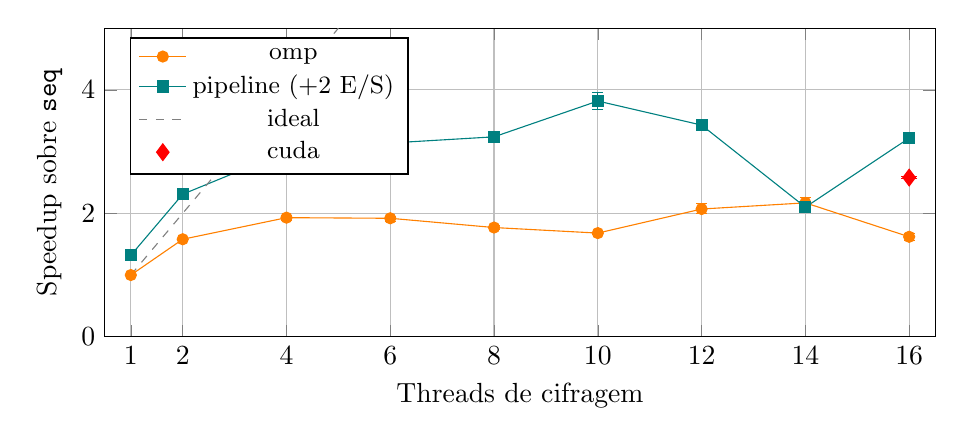
\begin{tikzpicture}
\begin{axis}[width=\linewidth, height=5.5cm, xlabel={Threads de cifragem},
  ylabel={Speedup sobre \texttt{seq}}, ymin=0, ymax=5, xmin=0.5, xmax=16.5,
  xtick={1,2,4,6,8,10,12,14,16}, legend pos=north west, grid=major,
  legend style={font=\small}, error bars/y dir=both, error bars/y explicit]
\addplot[color=orange, mark=*] coordinates
 {(1,1.00) += (0,0.01) -= (0,0.00) (2,1.58) += (0,0.00) -= (0,0.01)
  (4,1.93) += (0,0.04) -= (0,0.04) (6,1.92) += (0,0.03) -= (0,0.05)
  (8,1.77) += (0,0.03) -= (0,0.03) (10,1.68) += (0,0.01) -= (0,0.02)
  (12,2.07) += (0,0.09) -= (0,0.07) (14,2.17) += (0,0.09) -= (0,0.08)
  (16,1.62) += (0,0.05) -= (0,0.06)};
\addplot[color=teal, mark=square*] coordinates
 {(1,1.32) += (0,0.00) -= (0,0.01) (2,2.31) += (0,0.02) -= (0,0.02)
  (4,3.00) += (0,0.02) -= (0,0.02) (6,3.14) += (0,0.03) -= (0,0.02)
  (8,3.24) += (0,0.04) -= (0,0.04) (10,3.82) += (0,0.14) -= (0,0.13)
  (12,3.43) += (0,0.07) -= (0,0.08) (14,2.10) += (0,0.06) -= (0,0.06)
  (16,3.22) += (0,0.02) -= (0,0.03)};
\addplot[dashed, gray, domain=1:5] {x};
\addplot[only marks, mark=diamond*, mark size=3pt, color=red] coordinates
 {(16,2.58) += (0,0.02) -= (0,0.02)};
\legend{omp, pipeline (+2 E/S), ideal, cuda}
\end{axis}
\end{tikzpicture}
\caption{Speedup total (média de 9 a 10 execuções; barras: IC95\% por
\textit{bootstrap}). O ponto \texttt{cuda} não corresponde a 16 threads.}
\label{fig:speedup}
\end{figure}

\begin{table}[ht]
\centering
\small
\caption{Desempenho -- 901 quadros em 1080p (média $\pm$ dp de $n$ execuções)}
\label{tab:desempenho}
\begin{tabular}{lrrrrr}
\hline
\textbf{Config.} & \textbf{$n$} & \textbf{T. total (s)} & \textbf{IC95\% (s)} &
\textbf{Speedup [IC95\%]} & \textbf{T. cifra (s)} \\
\hline
\texttt{seq}           & 10 & 12,10 $\pm$ 0,05 & [12,06; 12,13] & 1,00 & 8,77 $\pm$ 0,02 \\
\texttt{omp 4}         & 10 & 6,25 $\pm$ 0,22 & [6,09; 6,41] & 1,93 [1,89; 1,97] & 3,14 $\pm$ 0,13 \\
\texttt{omp 8}         & 10 & 6,84 $\pm$ 0,17 & [6,72; 6,97] & 1,77 [1,74; 1,80] & 2,19 $\pm$ 0,02 \\
\texttt{omp 14}        & 9  & 5,58 $\pm$ 0,36 & [5,30; 5,85] & 2,17 [2,09; 2,26] & 2,05 $\pm$ 0,12 \\
\texttt{omp 16}        & 10 & 7,45 $\pm$ 0,44 & [7,14; 7,77] & 1,62 [1,56; 1,67] & 4,05 $\pm$ 0,43 \\
\texttt{pipeline 4+2}  & 10 & 4,03 $\pm$ 0,05 & [3,99; 4,06] & 3,00 [2,98; 3,02] & 3,62 $\pm$ 0,07 \\
\texttt{pipeline 8+2}  & 10 & 3,74 $\pm$ 0,07 & [3,69; 3,79] & 3,24 [3,20; 3,28] & 2,30 $\pm$ 0,03 \\
\texttt{pipeline 10+2} & 10 & \textbf{3,17} $\pm$ 0,19 & [3,03; 3,30] & \textbf{3,82} [3,69; 3,96] & 2,09 $\pm$ 0,05 \\
\texttt{pipeline 14+2} & 9  & 5,77 $\pm$ 0,26 & [5,57; 5,97] & 2,10 [2,04; 2,16] & 2,96 $\pm$ 0,11 \\
\texttt{pipeline 16+2} & 10 & 3,76 $\pm$ 0,05 & [3,73; 3,80] & 3,22 [3,19; 3,24] & 1,34 $\pm$ 0,03 \\
\texttt{cuda}          & 10 & 4,69 $\pm$ 0,05 & [4,65; 4,72] & 2,58 [2,56; 2,60] & 1,51 $\pm$ 0,04 \\
\hline
\end{tabular}
\par\smallskip
{\footnotesize\textit{Nota:} na \texttt{cuda}, T.\ cifra inclui as cópias entre
CPU e GPU (Tabela~\ref{tab:escopo}). Os demais números de threads estão na
Figura~\ref{fig:speedup} e no repositório.}
\end{table}

\subsection{Desempenho com GPU}

O \texttt{cuda} completou o vídeo em 4,69 $\pm$ 0,05 s (2,58$\times$), dos
quais 0,19 s foram de criação do contexto da GPU. Sua cifragem, de
1,51 $\pm$ 0,04 s, foi 5,81$\times$ mais rápida que a do \texttt{seq}, mas
apenas 0,10 s correspondeu ao \textit{kernel}: as cópias CPU$\to$GPU
(0,69 s) e GPU$\to$CPU (0,62 s) ocuparam 87\% dela. Com a cifragem reduzida, o
tempo passa a ser dominado pela gravação no \textit{pipe} de saída
(2,03 $\pm$ 0,01 s), que não acelera com a GPU. No mesmo escopo de
$T_{\mathrm{total}}$, o \texttt{pipeline 10+2} foi 32\% mais rápido que o
\texttt{cuda} ($p < 0{,}001$), enquanto o melhor \texttt{omp} foi 19\% mais
lento que o \texttt{cuda} ($p < 0{,}001$): para esta carga, a E/S é o gargalo, e sobrepor as etapas é mais
eficaz do que acelerar só a cifragem. Isso sugere que combinar o
\texttt{pipeline} com a cifragem em GPU é promissor.

\subsection{Eficiência energética}

A Tabela~\ref{tab:energia} mostra a energia na janela de $T_{\mathrm{total}}$.
A potência média do pacote da CPU subiu de 35,2 W no \texttt{seq} para até
72,6 W no \texttt{pipeline 10+2}, mas a energia caiu, porque o tempo caiu mais.
Na energia bruta de CPU e GPU, o \texttt{pipeline 10+2} foi o mais econômico
(251 $\pm$ 12 J; 0,278 J por quadro), 9,1\% abaixo do \texttt{cuda}
($p < 0{,}001$) e empatado com o \texttt{pipeline 12+2} ($p = 0{,}06$); como
também foi o mais rápido, teve o menor EDP. Na energia líquida, porém, o
\texttt{cuda} foi o mais econômico (140 $\pm$ 6 J, contra 159 $\pm$ 8 J do
\texttt{pipeline 10+2}; $p < 0{,}001$): a cifragem na GPU acrescenta pouca
potência acima do repouso, enquanto o \texttt{pipeline} economiza sobretudo por
terminar antes e acumular menos consumo de base. A versão mais eficiente
depende, portanto, de se contar ou não a potência de repouso da plataforma.

\begin{table}[ht]
\centering
\small
\caption{Energia na janela de $T_{\mathrm{total}}$ (média $\pm$ dp de $n$
execuções; $n$ como na Tabela~\ref{tab:desempenho})}
\label{tab:energia}
\begin{tabular}{lrrrrrr}
\hline
\textbf{Config.} & \textbf{$P_{\mathrm{CPU}}$ (W)} & \textbf{$E_{\mathrm{CPU}}$ (J)} &
\textbf{$E_{\mathrm{GPU}}$ (J)} & \textbf{$E_{\mathrm{CPU+GPU}}$ (J)} &
\textbf{Líquida (J)} & \textbf{J/quadro} \\
\hline
\texttt{seq}           & 35,2 & 426 $\pm$ 5  & 79 $\pm$ 0 & 504 $\pm$ 5  & 154 $\pm$ 5  & 0,560 \\
\texttt{omp 4}         & 54,7 & 343 $\pm$ 24 & 40 $\pm$ 1 & 383 $\pm$ 26 & 201 $\pm$ 20 & 0,425 \\
\texttt{omp 8}         & 58,4 & 399 $\pm$ 9  & 44 $\pm$ 1 & 443 $\pm$ 9  & 245 $\pm$ 6  & 0,492 \\
\texttt{omp 14}        & 62,4 & 348 $\pm$ 19 & 36 $\pm$ 3 & 384 $\pm$ 21 & 222 $\pm$ 12 & 0,426 \\
\texttt{omp 16}        & 58,7 & 437 $\pm$ 27 & 47 $\pm$ 3 & 484 $\pm$ 30 & 268 $\pm$ 17 & 0,537 \\
\texttt{pipeline 4+2}  & 68,4 & 275 $\pm$ 12 & 26 $\pm$ 1 & 301 $\pm$ 13 & 185 $\pm$ 11 & 0,334 \\
\texttt{pipeline 8+2}  & 70,9 & 265 $\pm$ 7  & 24 $\pm$ 1 & 289 $\pm$ 7  & 181 $\pm$ 7  & 0,321 \\
\texttt{pipeline 10+2} & 72,6 & 230 $\pm$ 11 & 21 $\pm$ 1 & \textbf{251} $\pm$ 12 & 159 $\pm$ 8 & \textbf{0,278} \\
\texttt{pipeline 14+2} & 61,8 & 356 $\pm$ 10 & 37 $\pm$ 2 & 393 $\pm$ 12 & 226 $\pm$ 6  & 0,436 \\
\texttt{pipeline 16+2} & 65,3 & 246 $\pm$ 9  & 25 $\pm$ 0 & 270 $\pm$ 10 & 161 $\pm$ 8  & 0,300 \\
\texttt{cuda}          & 46,8 & 220 $\pm$ 6  & 56 $\pm$ 1 & 275 $\pm$ 6  & \textbf{140} $\pm$ 6 & 0,306 \\
\hline
\end{tabular}
\end{table}

No \texttt{omp}, o resultado difere da hipótese inicial. A energia bruta ficou
empatada entre 2, 4 e 14 threads (391, 383 e 384 J; $p \geq 0{,}68$), e 14
threads, acima dos 10 núcleos físicos, deu o menor tempo do modo sem custo
energético adicional. Já 8, 10 e 16 threads foram mais lentas e gastaram mais
energia que 14 ($p < 0{,}05$); em particular, 16 threads consumiu 8,6\% mais que
8 ($p = 0{,}01$) e ainda foi mais lenta. Na energia líquida, o menor consumo do
modo ocorreu com 1 e 2 threads (160 e 168 J, empatados), 24\% abaixo de 14
threads ($p < 0{,}001$): acima do repouso, as threads adicionais reduziram o
tempo, mas acrescentaram mais energia do que economizaram, o que é compatível
com a parte da hipótese que previa aumento de consumo sem ganho proporcional de
desempenho.

\subsection{Efeito do descarte da saída}
\label{sec:sensibilidade}

Para avaliar se o descarte da saída altera a comparação, seis configurações
foram repetidas três vezes na mesma sessão, primeiro com a saída descartada e
depois gravando o vídeo cifrado em disco (Tabela~\ref{tab:disco}). Com o disco,
todas as versões paralelas ficaram entre 8,0 e 9,5 s, o que corresponde a gravar
2,8 GB a cerca de 300--350 MB/s: o tempo passa a ser limitado pela escrita no
disco, e quanto mais rápida a versão, mais ela espera por ele. A variação
também aumentou (coeficiente de variação de até 52\% no \texttt{cuda}), e
nenhuma diferença entre versões paralelas foi significativa ($p_{\mathrm{Holm}}
= 1{,}0$), enquanto, com a saída descartada, o \texttt{pipeline 10+2} superou o
\texttt{cuda} e o \texttt{omp 10} ($p < 0{,}01$). A única conclusão presente
nos dois casos, a de que todas as versões paralelas superam o \texttt{seq}, se
manteve. Incluir o disco, portanto, não revelaria outra ordem entre as
estratégias, mas substituiria a comparação entre elas pela medida de um
gargalo de \textit{hardware} comum a todas; o descarte preserva a comparação ao
manter o \textit{pipe} de saída e remover apenas esse limite.

\begin{table}[ht]
\centering
\small
\caption{Tempo total com a saída descartada e gravada em disco (média $\pm$ dp
de 3 execuções)}
\label{tab:disco}
\begin{tabular}{lrr}
\hline
\textbf{Config.} & \textbf{Descartada (s)} & \textbf{Em disco (s)} \\
\hline
\texttt{seq}           & 12,27 $\pm$ 0,04 & 12,73 $\pm$ 0,08 \\
\texttt{omp 10}        & 7,41 $\pm$ 0,05  & 8,04 $\pm$ 0,47 \\
\texttt{omp 14}        & 6,08 $\pm$ 0,94  & 9,02 $\pm$ 0,34 \\
\texttt{pipeline 10+2} & 3,33 $\pm$ 0,21  & 8,69 $\pm$ 2,79 \\
\texttt{pipeline 14+2} & 6,04 $\pm$ 0,31  & 9,53 $\pm$ 0,58 \\
\texttt{cuda}          & 4,93 $\pm$ 0,14  & 8,66 $\pm$ 4,48 \\
\hline
\end{tabular}
\end{table}

\subsection{Qualidade criptográfica}

Em um quadro cifrado com a semente 123, a entropia dos planos Y, U e V subiu de
6,04--6,91 para 7,90--7,99 bits e a correlação entre pixels vizinhos caiu de
0,94--0,96 para no máximo 0,017. O plano U apresentou vazamento visível, devido
à linearidade da cifra em regiões de crominância neutra.


% =============================================================================
\section{Ameaças à Validade}
% =============================================================================

Os resultados vêm de uma única plataforma e não se generalizam diretamente a
outras arquiteturas: o i5-13450HX combina núcleos de desempenho e de
eficiência, cuja ocupação fica a cargo do sistema operacional, e a vantagem do
\texttt{pipeline} sobre o \texttt{cuda} vale para a GPU avaliada e para uma
carga dominada por E/S, podendo se inverter com GPUs mais rápidas ou cargas de
cifragem mais pesadas. A execução no WSL~2 acrescenta a camada de
virtualização do Windows, igual para todas as versões, de modo que os tempos
absolutos podem diferir de um Linux nativo. Outros processos do sistema e a
temperatura do notebook introduzem variabilidade, mitigada, mas não eliminada,
pela ordem embaralhada, pelas pausas e pelas repetições; seis configurações
tiveram 9 em vez de 10 repetições. Quanto à energia, a amostragem de 100 a
110 ms, para execuções de 3 a 12 s, deixa imprecisão residual nos limites da
janela; RAPL e \texttt{nvidia-smi} são estimativas dos próprios componentes, a
potência de repouso foi medida em uma única janela de 30 s, e nenhum dos dois
domínios cobre memória, tela ou armazenamento. O efeito da gravação em disco
foi avaliado com apenas três repetições por configuração, suficientes para
mostrar a perda de resolução entre as versões, mas não para estimá-la com
precisão. Por fim, a Cifra de Hill tem finalidade experimental, e seu vazamento
em regiões uniformes não invalida as conclusões sobre desempenho e energia.


% =============================================================================
\section{Conclusão}
% =============================================================================

Este trabalho investigou o impacto do número de threads no desempenho e na
eficiência energética da Cifra de Hill em memória compartilhada, com tempo e
energia medidos no mesmo escopo para todas as versões. Em desempenho, o
\texttt{pipeline} obteve o maior speedup total (3,82$\times$ com 10 threads de
cifragem), superando significativamente a versão \texttt{cuda}, cuja cifragem
foi dominada pelas cópias entre CPU e GPU; o speedup da cifragem isolada
superou o total em todas as versões paralelas, o que evidencia a E/S como
gargalo, em linha com a Lei de Amdahl. Mais threads não reduziram o tempo de
forma contínua: o \texttt{omp} teve o melhor resultado com 14 threads e piorou
com 16, padrão compatível com a combinação de núcleos de desempenho e
eficiência. Em energia, a configuração mais rápida também foi a de menor energia
bruta de CPU e GPU, mas o \texttt{cuda} teve a menor energia acima do repouso,
o que reforça a importância de analisar desempenho e consumo em conjunto e de
explicitar o que entra em cada medida.

Como trabalhos futuros, pretende-se repetir os experimentos em Linux nativo e em
outras arquiteturas, fixar as threads em núcleos de desempenho ou de eficiência
para isolar o efeito da arquitetura híbrida, medir o consumo total com um
medidor externo, avaliar a combinação do \texttt{pipeline} com a cifragem em GPU
e investigar uma extensão afim da cifra para eliminar o vazamento em regiões
uniformes.


\bibliographystyle{sbc}
\bibliography{sbc-template}

\end{document}
